\chapter{Constrained Clustering}\label{ch:ConstrainedClustering}

Having introduced the basic concepts of clustering, the aim of this chapter is to define the concepts related to constrained clustering, as well as to give examples of its application and highlight the benefits and problems presented by its use. To this end we take as our main reference the survey presented in \cite{davidson2007survey}.

\section{Motivation for Constrained Clustering}

As we discussed in Chapter \ref{ch:IntroClustering}, unsupervised clustering methods are useful for structuring data referring to a particular area. An example of this can be found in text classification; In \cite{cohn2003semi} a problem proposed by Yahoo! is faced. The problem consist of, given a large number of text documents, grouping them according to a taxonomy in which documents with similar topics are nearby. For this, unsupervised clustering methods are useful, as the information on the problem initially available is limited. However, in \cite{wagstaff2001constrained} is shown that applying unsupervised clustering to certain problems, such as grouping GPS data in such a way that clusters define the lanes of a road, does not produce significant results, as the clusters obtained are far from the elongated shape that would be expected as a result. To tackle the problem, they introduced a new element in clustering, the instance-level constraints, which made it possible to include knowledge about the clusters that would guide the clustering methods to obtain the expected results. It was enough to indicate that the lanes of the road on which the vehicles circulate are four meters wide, and therefore any vehicle that is at a distance of more than 4 meters from another, perpendicular to the direction of displacement, must be located in a different cluster.

We are now in a new scenario: it is possible to incorporate additional information to the clustering process, in addition to that contained in the data set itself, to guide it in the formation of the partition and obtain more precise results. This places constrained clustering in the framework of semi-supervised learning, unlike traditional clustering methods which fall within the area of unsupervised clustering. 

\section{Constraints Definition}

The new type of information that we incorporate to clustering is given in the form of instance-level constraints, that is, to specify if two instances ($x_i$ and $x_j$) from the dataset ($X$) must be in the same cluster or, on the contrary, they must be in separate clusters.

Constraints that indicate that two instances must be placed in the same cluster are called \acf{ML}, and are noted with $C_=(x_i,x_j)$. Similarly, constraints that specify that two instances must not be placed in the same cluster are called \acf{CL}, and are noted with $C_\neq(x_i,x_j)$ \cite{wagstaff2000clustering}.

Although they may seem simple, constraints defined as above have some very interesting properties. Must-link constraints are an example of an equivalence relationship, and therefore are symmetrical, reflexive and transitive, formalizing:

\begin{observation}
	\textbf{Must-link constraints are transitive.} Let $CC_i$ and $CC_j$ be connected components (completely connected subgraphs by \acs{ML} constraints), and let $x_i$ and $x_j$ be the instances in $CC_i$ and $CC_j$ respectively. Then $C_=(x,y): x \in CC_i, y \in CC_j \rightarrow C_=(a,b) \forall a,b: a\in CC_i, b \in CC_j$. \cite{davidson2007survey}
\end{observation}

\begin{observacion}
	\textbf{Cannot-link constraints can be entailed.} Let $CC_i$ and $CC_j$ be connected components (completely connected subgraphs by \acs{CL} constraints) and let $x_i$ and $x_j$ be the instances in $CC_i$ and $CC_j$ respectively. Then $C_\neq(x,y): x \in CC_i, y \in CC_j \rightarrow _\neq(a,b) \forall a,b: a\in CC_i, b \in CC_j$. \cite{davidson2007survey}
\end{observacion}

A clear example of constraint use can be found in clustering applications where there are distance measurement limitations, as in the case of GPS data. Thus, if we want that instances forming two clusters to be separated by a distance greater or equal to $\delta$, it is enough to set \acs{ML} constraints between all instances separated by less than $\delta$ units. Similarly, if we want the diameter of the clusters to be at most $\epsilon$, we must set \acs{CL} constraint between instances separated by more than $\epsilon$ units. Figure \ref{fig:DistanceConstraints} shows a graphical representation of these two types of constraints.

\begin{figure}[!h]
	\centering
	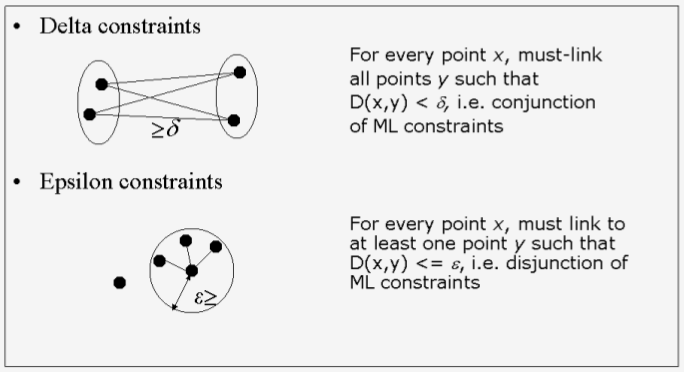
\includegraphics[scale=0.45]{gfx/ConstClust/RestriccionesDeltaEpsilon.png} 
	\caption[\textit{delta} and \textit{epsilon} constraints]{\textit{delta} and \textit{epsilon} constraints \cite{davidson2007survey}.}\label{fig:DistanceConstraints}
\end{figure}


\section{Use of Constraints}

While supervised learning involves knowing the label associated with each instance, \acf{SSL} has only a subset of tagged instances. On the other hand, in many domains the available information refers to relations between instances, and not to the specific class to which they belong. Moreover, in interactive clustering systems, a user who is not expert in the domain of the problem will probably be able to provide information in the form of constraints such as \acf{ML} and \acf{CL}. \cite{cohn2003semi}\cite{davidson2007hierarchical}, rather than providing information on what particular class certain instances belong to.

Typically, constraints are incorporated into clustering problems in two ways. They can be used to alter the instance clusters assignment rule of the method in hand, so that the solution satisfies as many constraints as possible. Alternatively, it is possible to train the distance function used by the method based on the constraints, either before or during the application of the method. In any case, the initialization phase can take the constraints into account, so that instances associated with constraints \acf{ML} will be placed in the same cluster, and those between which there is a constraint \acf{CL} will be placed in different clusters. Based on this distinction, we identify two ways of approaching the problem, those based on constraints (\textit{constraint-based}), and those based on distances (\textit{distance-based}).

\subsection{Constraints-based Methods}

In constraint-based methods, the clustering method itself is modified in such a way that the available information is used to bias the search and obtain an appropriate data partition.

Regarding the degree to which the constraints have to be satisfied, we can make a distinction between the concepts of hard \cite{wagstaff2001constrained}\cite{davidson2005agglomerative} and soft \cite{law2004clustering}\cite{basu2004active}\cite{segal2003discovering}\cite{davidson2005clustering}\cite{law2005model} constraints. Hard constraints must necessarily be satisfied in the output partition of any algorithm that makes use of them, while soft constraints are taken as a strong guide for the algorithm that uses them but can be partially satisfied in the output partition \cite{seret2014new}. For the purposes of this work, we will employ the latter. There are several techniques to obtain a partition based on constraints:

\begin{itemize}
	
	\item  Modify the objective function to include a penalty term for breaking constraints \cite{demiriz1999semi} \cite{davidson2005clustering}.
	
	\item Group instances with additional information obtained from a conditional distribution into an auxiliary space \cite{sinkkonen2000semisupervised}.
	
	\item Enforcing all constraints to be satisfied by modifying the the instance clusters assignment rule \cite{wagstaff2001constrained}.
	
	\item Initialize clusters based on constraints inferred from a set of labeled instances \cite{basu2002semi}.
	
\end{itemize}

Figure \ref{fig:ConstOverDataset} shows a data set together with its associated constraints. Figure \ref{fig:ClusteringSatAllConst} proposes a possible clustering that satisfies all constraints.

\begin{figure}[bth]
	\myfloatalign
	{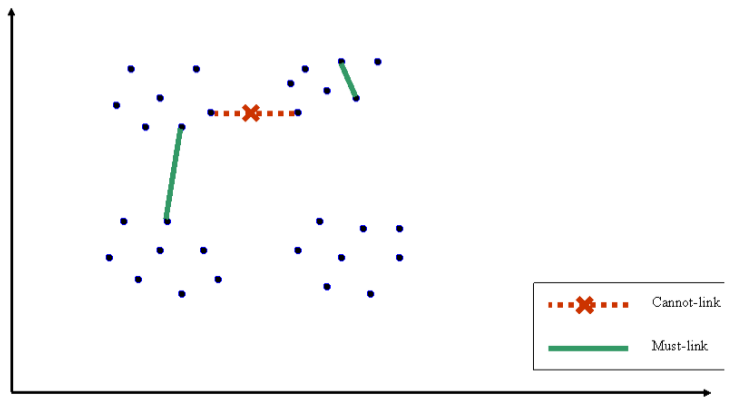
\includegraphics[width=.6\linewidth]{gfx/ConstClust/InputInstancesAndConst1}
	\caption[Constraints on a dataset.]{Constraints on a dataset. \cite{davidson2007survey}} \label{fig:ConstOverDataset}
	}
	{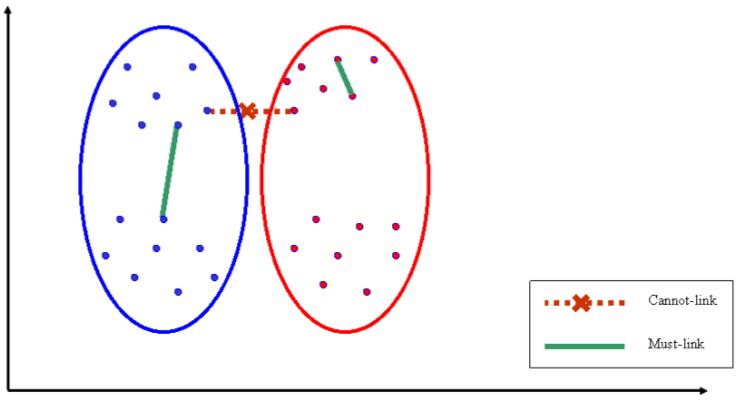
\includegraphics[width=.6\linewidth]{gfx/ConstClust/ClusteringSatAll}
	\caption[Clustering satisfying all constraints.]{Clustering satisfying all constraints. \cite{davidson2007survey}} \label{fig:ClusteringSatAllConst}
	}
\end{figure}

\subsection{Distance-based Methods}

In distance-based approaches, classic clustering methods that use a distance measurement are employed, so that the distance measurement is modified to incorporate the constraints. In this context, satisfying constraints means that instances related to constraints \acf{ML} are placed together in the space, and those related by \acf{CL} are separated.

Figure \ref{fig:MetricLearned} shows a possible clustering based on a metric learned from the constraints specified in Figure \ref{fig:ConstOverDataset2}. It should be noted that in Figure \ref{fig:MetricLearned} the space in which the data is located has been compressed on the vertical axis and widened on the horizontal axis to match the learned distance metric.

\begin{figure}[bth]
	\myfloatalign
	{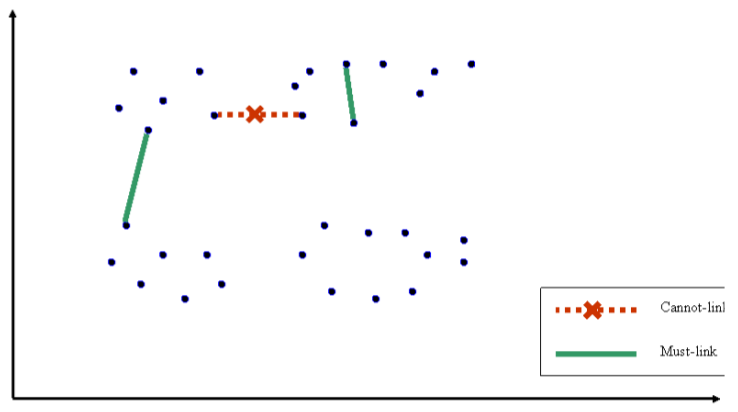
\includegraphics[width=.6\linewidth]{gfx/ConstClust/InputInstancesAndConst2}
	\caption[Constraints on a dataset.]{Constraints on a dataset. \cite{davidson2007survey}} \label{fig:ConstOverDataset2}
	}
	{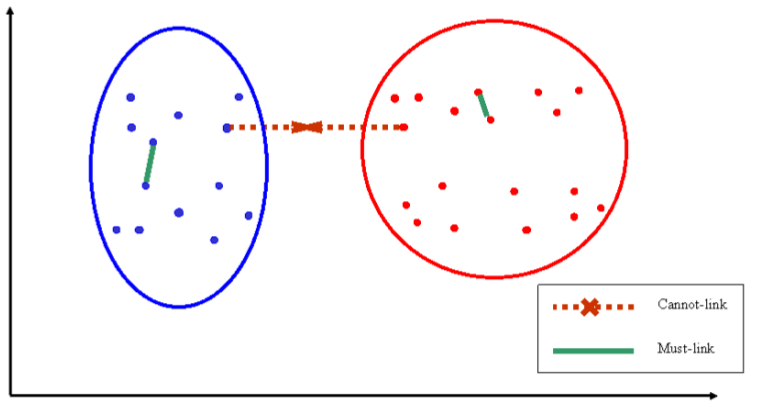
\includegraphics[width=.6\linewidth]{gfx/ConstClust/MetricaAprendida}
	\caption[Clustering based on a metric learned based on constraints.]{Clustering based on a metric learned based on constraints. \cite{davidson2007survey}} \label{fig:MetricLearned}
	}
\end{figure}

\section{Constrained Clustering Applications} \label{sec:CCApplications}

This section shows some application cases in which constrained clustering has turned out to be a more useful tool than unsupervised clustering. For each case we will analyze how the constraints were obtained and how they improve the results in the resulting clustering. 

\subsection{Image Analysis}

Figure \ref{fig:CMUFacesDatabase} shows a sample from the CMU (Carnegie Mellon University) faces dataset, where the task is to group faces based on different criteria. In this case, the goal is to group the faces according to their orientation.

\clearpage

\begin{figure}[bth]
	\myfloatalign
	\subfloat[Profile faces.]
	{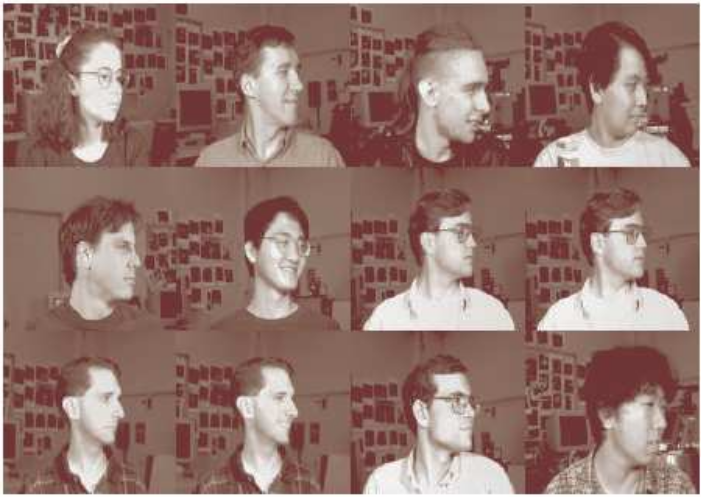
\includegraphics[width=.3\linewidth]{gfx/ConstClust/AnalisisImagenes/Caras1}} \quad
	\subfloat[Front faces.]
	{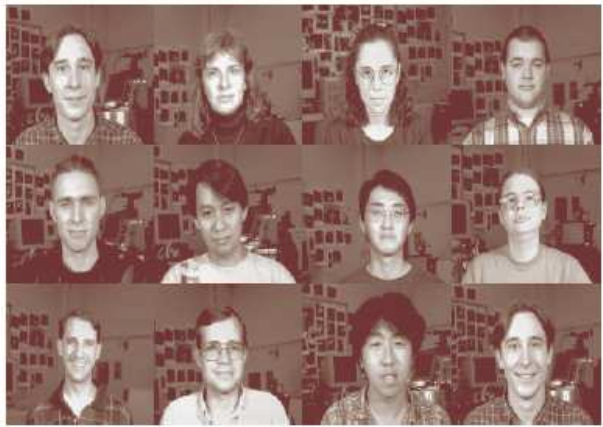
\includegraphics[width=.3\linewidth]{gfx/ConstClust/AnalisisImagenes/Caras3}} \quad
	\subfloat[Faces up.]
	{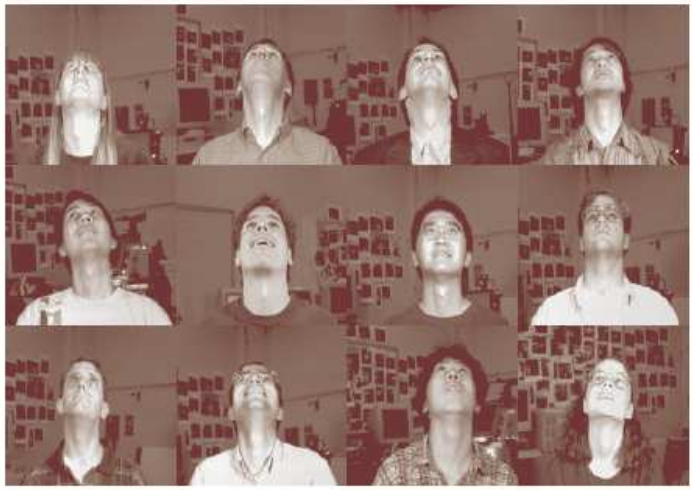
\includegraphics[width=.3\linewidth]{gfx/ConstClust/AnalisisImagenes/Caras2}} \quad
	\caption[CMU database faces.]{CMU database faces. \cite{davidson2007survey}}\label{fig:CMUFacesDatabase}
\end{figure}

The method used to obtain the constraints is one of the most popular in the literature: set the number of clusters of the resulting partition equal to the number of classes in the database, and generate the constraints from a subset of tagged instances; that is, if two instances have different labels, set a \acf{CL} constraint between them, otherwise one of \acf{ML} type. Thus, between the images shown in Figure \ref{fig:CMUFacesDatabase} \acf{CL} constraints are set, since, although they belong to the same person, they do not have the same orientation.

\begin{figure}[bth]
	\myfloatalign
	{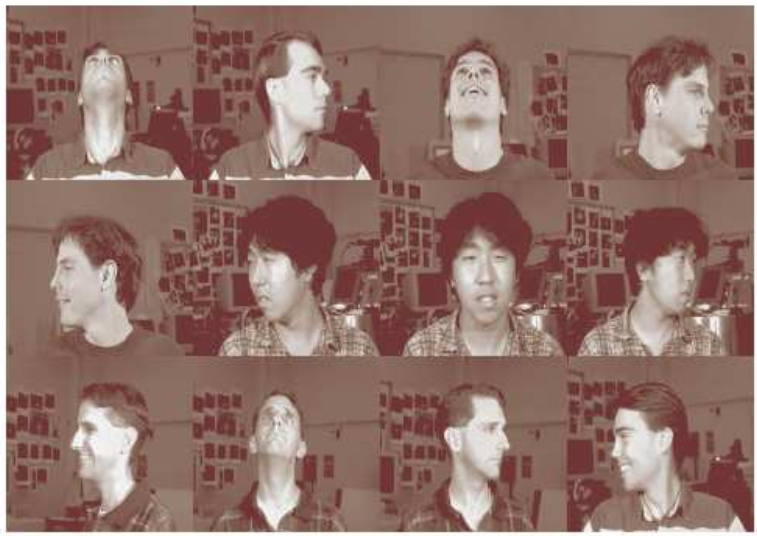
\includegraphics[width=.35\linewidth]{gfx/ConstClust/AnalisisImagenes/CarasDifOr1}} \quad
	{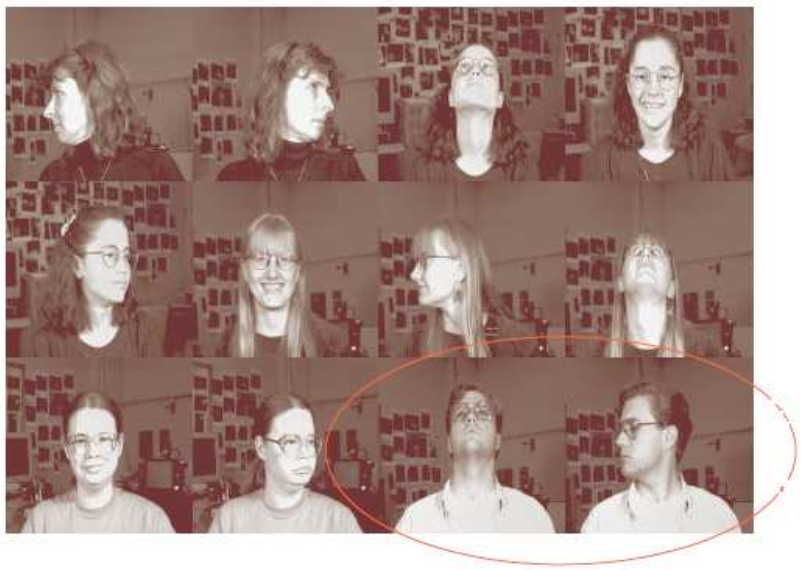
\includegraphics[width=.35\linewidth]{gfx/ConstClust/AnalisisImagenes/CarasDifOr2}}
	\caption[\acs{CL} constraints between faces of the same person.]{\acs{CL} constraints between faces of the same person. \cite{davidson2007survey}}\label{fig:figure10}
\end{figure}

Figure \ref{fig:AiboRoboRobtoClustSys} shows another set of image data on which constrained clustering techniques are applied. In this case, the task is to perform object recognition to incorporate the method into the navigation system of the Aibo robot \cite{davidson2005clustering}. Distance constraints such as $\delta$ and $\epsilon$ are used as described in Figure \ref{fig:DistanceConstraints}. In this way well differentiated clusters are obtained and therefore they are useful for the path-finding techniques performed by the robot during navigation.

\begin{figure}[bth]
	\myfloatalign
	\subfloat[Imagen original]
	{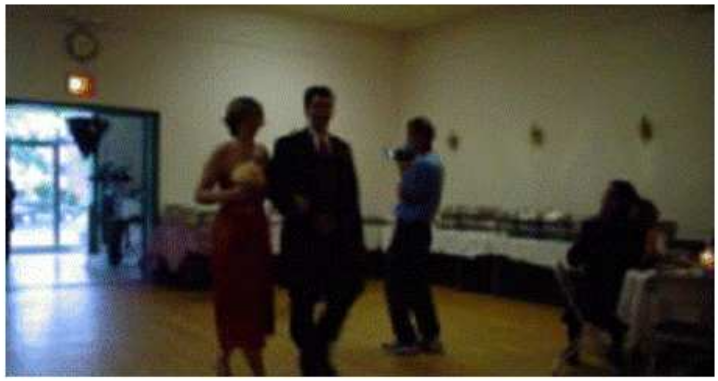
\includegraphics[width=.3\linewidth]{gfx/ConstClust/AnalisisImagenes/Aibo1}} \quad
	\subfloat[Clustering sin restricciones]
	{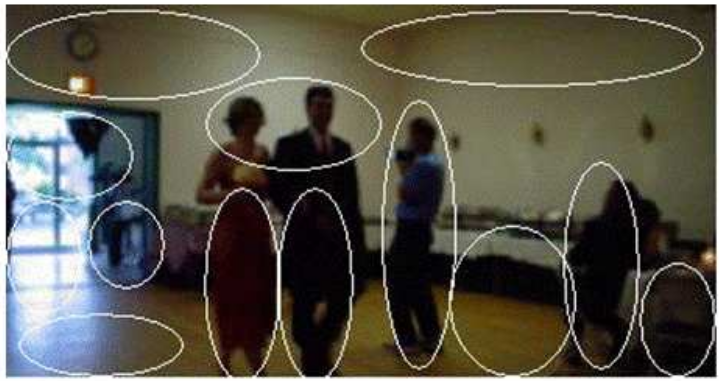
\includegraphics[width=.3\linewidth]{gfx/ConstClust/AnalisisImagenes/Aibo2}} \quad
	\subfloat[Clustering con restricciones]
	{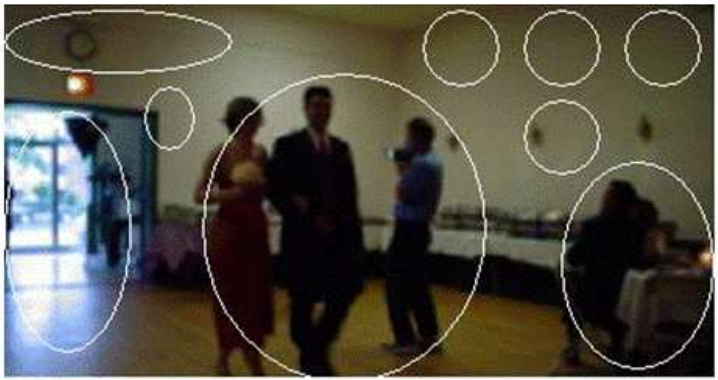
\includegraphics[width=.3\linewidth]{gfx/ConstClust/AnalisisImagenes/Aibo3}} \quad
	\caption[Clustering method used in Aibo Robot navigation system.]{Clustering method used in Aibo Robot navigation system. \cite{davidson2007survey}\cite{davidson2005clustering}}\label{fig:AiboRobtoClustSys}
\end{figure}

\subsection{Video Analysis}

Video databases are one example where constraints can be generated directly from the data domain, especially if space-time data information is available \cite{yan2006discriminative}. In time sequenced data it is possible to set \acf{ML} constraints between groups of pixels of frames close in time. This is especially useful when the task is to perform object recognition based on clustering and segmentation. It is also possible to add \acf{CL} constraints to image segment in the same snapshot, as there is a low probability that they are associated with the same object after segmentation is done. In fact, in the video analysis domain problems there are a variety of constraint extraction methods \cite{yan2006discriminative}, Figure \ref{fig:ConstExtractionVideo} shows some examples. 

\begin{figure}[bth]
	\myfloatalign
	\subfloat[]
	{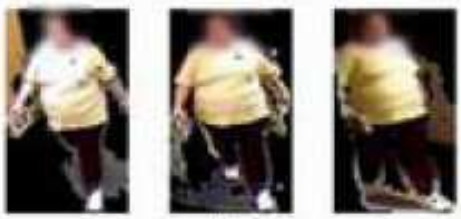
\includegraphics[width=.4\linewidth]{gfx/ConstClust/Videos/VideoA}}
	\quad
	\subfloat[]
	{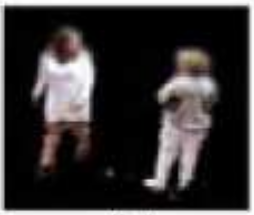
\includegraphics[width=.225\linewidth]{gfx/ConstClust/Videos/VideoB}} \quad
	\subfloat[]
	{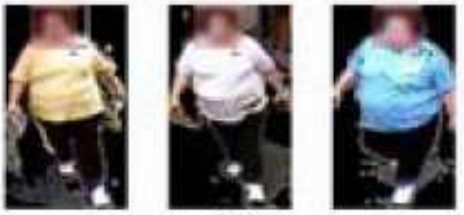
\includegraphics[width=.4\linewidth]{gfx/ConstClust/Videos/VideoC}}
	\quad
	\subfloat[]
	{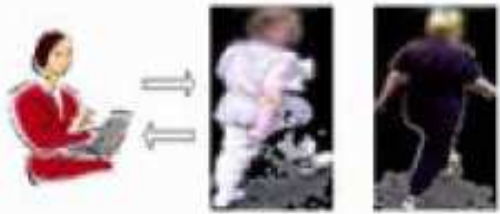
\includegraphics[width=.4\linewidth]{gfx/ConstClust/Videos/VideoD}}
	\caption[Constraints extraction in video data.]{Constraints extraction in video data. \cite{yan2006discriminative} \cite{davidson2007survey}}\label{fig:ConstExtractionVideo}
\end{figure}

In Figure \ref{fig:ConstExtractionVideo}, image (a) corresponds to constraints extracted from tracking a person over a period of time, (b) corresponds to spatial constraints associating two objects located in the same frame, image (c) corresponds to restrictions obtained through facial recognition and (d) to those provided by the user.

With so many constraint extraction methods, one might ask: what happens if too many constraints are imposed? Does this make the problem over-constrained? In Section \ref{sec:CCDisadvantages} we will address these questions.

\subsection{Biological Data}

In gene clustering based on micro-array data, genes are represented by their expression profile in different experiments and grouped using different methods, in this case constrained clustering methods. Figure \ref{fig:GeneticApp} shows an example: these are \acf{ML} constraints set between genes based on co-occurrence data stored in the protein interaction database, which contains information about which genes (and their associated proteins) are present in the same cell processes \cite{xenarios2001dip}. This information can be used to improve results provided by clustering methods. \cite{segal2003discovering}.

\begin{figure}[!h]
	\centering
	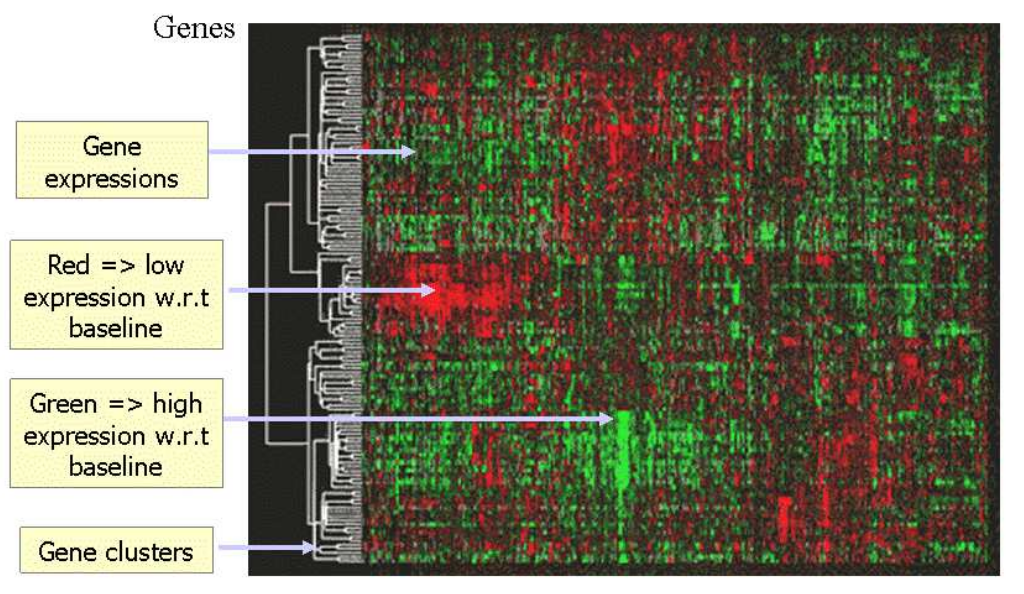
\includegraphics[scale=0.3]{gfx/ConstClust/Genetica/Genes} 
	\caption[Gene clustering based on micro-array data.]{Gene clustering based on micro-array data. \cite{davidson2007survey}}\label{fig:GeneticApp}
\end{figure}

\subsection{Text Analysis}

In content classification tasks, the goal is to automatically split large amounts of documents into groups or clusters. In this case it is possible to extract constraints from multiple auxiliary resources. For example, if two documents are in the same directory, a \acf{ML} constraints could be set between them. This way it is possible to adjust the resulting clustering to suit a particular criterion, such as creating a hierarchy of documents similar to the way they are organized in the input directories structure.

\subsection{Web Data} 

El clustering con restricciones resulta de gran utilidad en el procesamiento de datos de búsqueda en páginas web. Aquí, el objetivo es agrupar, de manera automática, los resultados de una consulta ambigua en el motor de búsqueda en clusters de \acs{URL}s, que se refieran al concepto introducido como consulta en diferentes contextos. En este ámbito es posible extraer las restricciones a partir de búsquedas realizadas anteriormente por los usuarios, de manera que se establece una restricción de tipo \acf{ML} entre \acs{URL}s visitadas en la misma sesión de usuario. Aplicar clustering utilizando estas restricciones puede ayudar a sesgar el resultado de las búsquedas hacia las preferencias del usuario.

\subsection{Aplicaciones en datos de audio}

Constrained clustering is very useful in the processing of search data on web pages. Here, the aim is to automatically group the results of an ambiguous query in the search engine into clusters of \acs{URL}s, which refer to the concept introduced as a query in different contexts. In this area it is possible to extract constraints from searches previously performed by users, so that a \acf{ML} constraint is set between visited \acs{URL}s in the same user session. Clustering using these constraints can help biasing search results towards user preferences.

\subsection{Aplicaciones en datos de GPS} \label{EjemploGPS}

As mentioned at the beginning of Chapter \ref{ch:ConstrainedClustering}, constrained clustering can be applied to \acs{GPS} data to identify the lane in which each vehicle is running, as shown in Figure \ref{fig:GPSClustData}. Each instance is represented by the position it occupies on the road in two-dimensional Cartesian coordinates $(x,y)$, obtained from \acs{GPS} data. Figure \ref{fig:figure15} graphically shows this representation of the data (note that multiple instances can refer to the same vehicle at different times).

\begin{figure}[!h]
	\centering
	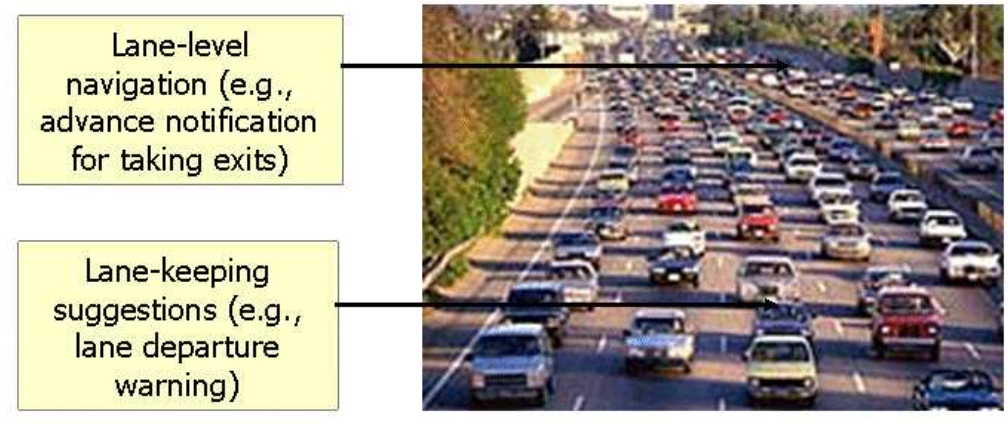
\includegraphics[scale=0.3]{gfx/ConstClust/GPS/Coches} 
	\caption[GPS data use.]{GPS data use. \cite{davidson2007survey} \cite{wagstaff2001constrained}}\label{fig:GPSClustData}
\end{figure}


In this domain, real clusters have an elongated shape on the horizontal axis and are aligned perpendicular to the motion direction. To get the resulting clusters to have this shape, we can make use of the constraints. We will set a \acf{CL} constraint between those instances more than 4 meters perpendicularly to the motion direction (since the lanes have a maximum width of 4 meters), and \acf{ML} constraints between those instances that present continuity in the motion direction axis, since it is likely that the vehicles they represent are in the same lane. This clustering model has proven to be very useful in real-time navigation \cite{wagstaff2001constrained}, allowing the user to be notified when to change lanes, or when not to leave them.

\begin{figure}[!h]
	\centering
	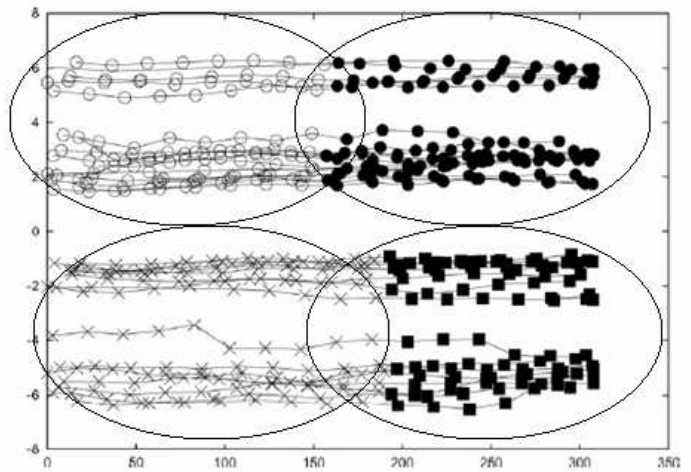
\includegraphics[scale=0.32]{gfx/ConstClust/GPS/Instancias} 
	\caption[Resulting Clustering from GPS data with no constraints.]{Resulting Clustering from GPS data with no constraints. \cite{davidson2007survey} \cite{wagstaff2001constrained}}\label{fig:figure15}
\end{figure}

\section{Beneficios del uso de restricciones}

Encontramos dos beneficios principales en el uso de restricciones: 

\begin{itemize}
	
	\item Incremento de la exactitud en las predicciones de las etiquetas al generar restricciones en base a un subconjunto de instancias etiquetadas.
	
	\item Obtención de clusters con geometría adaptable a cada problema.
	
\end{itemize}

A continuación se analizan estos dos beneficios:

Dado $X = \{x_1 \cdots x_u\}$, un gran conjunto de instancias no etiquetadas, y $L = \{(x_{u+1}, y_{u+1})\cdots (x_{u+l}, y_{u+l})\}$, un pequeño conjunto de instancias etiquetadas, es común escoger dos elementos de $L$ (con reemplazamiento) y establecer una restricción \acs{ML} entre ellos si pertenecen a la misma clase o, en caso contrario, una de tipo \acs{CL}. Un método apropiado para evaluar los resultados ofrecidos por un método de clustering es medir el nivel de exactitud de éste a la hora de predecir las etiquetas del conjunto $X$. Esto normalmente requiere que se especifique el número de clusters deseados igual al número de clases conocidas en $X$ ($K = K^*$). Para medir la exactitud se emplean métodos como \textit{Rand Index} \cite{rand1971objective}.

El trabajo de Wagstaff y Cardie \cite{wagstaff2000clustering}, en el que generaban las restricciones de la manera descrita anteriormente, demostraba que, cuando se realiza un promedio de la exactitud de las predicciones obtenidas con algoritmos de clustering con restricciones, variando estas últimas entre experimentos, se obtienen resultados hasta un 20\% mejores que con las técnicas clásicas.

\begin{observacion}
	
	\textbf{El uso de restricciones, en promedio, incrementa la precisión.}
	El rendimiento de un método al predecir etiquetas aumenta cuando se promedia empleando numerosos conjuntos de restricciones diferentes. \cite{davidson2007survey}
	\label{ob:observacion33}
	
\end{observacion}

Esta regla, sin embargo, no es cierta en todos los casos, pues en conjuntos de datos como \textit{Tic-Tac-Toe Endgame}, no se consigue ningún incremento en las predicciones sea cual sea el número de restricciones empleadas. La explicación dada por los autores citados para estas excepciones se basa en que establecer $K = K^*$ no es apropiado en este caso.

El otro beneficio que reporta el uso de restricciones es la posibilidad de obtener clusters con la geometría deseada, como el ejemplo de aplicar clustering a datos \acs{GPS}, analizado en la Sección \ref{EjemploGPS} de este trabajo.

\section{Problemas del uso de restricciones} \label{Problemas}

Aunque, tal y como hemos comprobado, la incorporación de restricciones a los métodos de clustering reporta beneficios en algunas aplicaciones, existen dos inconvenientes principales que se exponen a continuación, así como posibles soluciones a los mismos.

\subsection{El problema de la factibilidad}

La introducción de restricciones en el clustering cambia el problema al que éste da solución, que pasa a ser: \textit{Encontrar la mejor partición que satisfaga todas las restricciones}. De esta manera, si aquellas no están bien especificadas o si los métodos de extracción son inadecuados, podemos encontrar que las restricciones se contradicen, lo que deriva en que no existe una asignación de instancias a clusters que las satisfaga todas. Por ejemplo, no existe asignación que satisfaga las restricciones $ML(x_1,x_2)$ y $CL(x_1,x_2)$, independientemente del valor de $K$. Lo mismo sucede para $K = 2$, y las restricciones $CL(x_1, x_2)$, $CL(x_2, x_3)$ y $CL(x_1, x_3)$. Formalizando, el problema de la factibilidad para problemas de clustering (no jerárquico) con restricciones viene definido por:

\begin{definicion}
	
	\textbf{Problema de la factibilidad para clustering con restricciones:} Dado un conjunto de datos $X$, un conjunto de restricciones $R$, un umbral superior $K_l$ y un umbral superior $K_u$ para el número de clusters resultantes, ¿Existe una partición de $X$ en bloques tal que $K_l \le K \le K_u$ y todas las restricciones en $R$ se satisfacen? \cite{davidson2005clustering} \cite{davidson2007survey}
	
\end{definicion}

La complejidad teórica del problema dependerá del tipo de restricciones que se combinen en él. La Tabla \ref{tab:tabla1} presenta, de manera resumida, la complejidad esperada en cada caso. 

\begin{table}[h]
	\centering
	\setlength{\arrayrulewidth}{1mm}
	\setlength{\tabcolsep}{10pt}
	\renewcommand{\arraystretch}{1}
	
	\rowcolors{2}{gray!25}{white}
	\begin{tabular}{ >{\centering\arraybackslash}m{4cm}  >{\centering\arraybackslash}m{4cm} }
		\hline
		\rowcolor{black}
		\multicolumn{2}{c}{\bf \color{white}{Complejidad del clustering con restricciones}}\\
		\hline
		\rowcolor{gray!50}
		\textbf{Restricciones} & \textbf{Complejidad} \\
		Restricciones $\delta$ & $\mathbf{P}$ \\
		Restricciones $\epsilon$ & $\mathbf{P}$ \\
		\acs{ML} y $\delta$ & $\mathbf{P}$ \\
		\acs{ML} y $\epsilon$ & $\mathbf{NP}$-completo \\
		$\epsilon$ y $\delta$ & $\mathbf{P}$ \\
		\acs{CL} y otra & $\mathbf{NP}$-completo \\
		\hline
		
	\end{tabular}
	\caption[Complejidad del problema del clustering en función del tipo de restricciones]{Complejidad del problema del clustering en función del tipo de restricciones. \cite{davidson2007survey}}
	\label{tab:tabla1}
\end{table}

Tal y como queda reflejado en la Tabla \ref{tab:tabla1}, la utilización de restricciones \acf{CL} eleva el nivel de complejidad del clustering a $\mathbf{NP}$-completo y, por tanto, el problema del clustering con restricciones es intratable. De manera intuitiva puede entenderse fácilmente que, si encontrar una sola partición que satisfaga las restricciones es un problema complejo, más complejo es aún encontrar la mejor. 

\begin{observacion}
	
	\textbf{Saber que existe una solución factible no nos ayuda a encontrarla.} Las consecuencias de este resultado sobre la complejidad del clustering con restricciones implican que, aun en caso de que exista una partición factible, no será fácil de encontrar, hablando en términos de complejidad algorítmica. \cite{davidson2007survey}
	\label{ob:observacion34}
	
\end{observacion} 

Los autores Wagstaff \cite{wagstaff2002intelligent} y Davidson y Ravi \cite{davidson2007hierarchical} muestran que aun especificando el número de clusters de salida igual al de clases verdaderas ($K = K*$), cosa que garantiza que existe una solución factible, algoritmos simples como la adaptación de K-medias (\acs{KM}, Apéndice \ref{ap:kmeans}) al clustering con restricciones (\textit{COP-K-means} \cite{wagstaff2001constrained}, Sección \ref{copkm}), pueden no converger debido al problema de la factibilidad.

\subsection{El problema de la utilidad de conjuntos de restricciones} \label{ProbRestr}

En el clustering con restricciones se asume que éstas son indicaciones que guían al algoritmo para encontrar la partición de los datos deseada. Entonces, está justificado pensar que, de cuanta más información adicional (restricciones) dispongamos, más cercano estará el resultado que obtengamos al que buscamos, tal y como la Observación \ref{ob:observacion33} afirmaba. Sin embargo, y a pesar de lo dispuesto en dicha observación, encontramos casos en los que, aun generando las restricciones sin ruido y en base a las etiquetas verdaderas, existen conjuntos de restricciones que, lejos de mejorar los resultados, los empeoran considerablemente \cite{davidson2006proceedings}. Esto parece estar en desacuerdo con la Observación \ref{ob:observacion33}, sin embargo, recordemos que en ella se hace referencia al caso medio, y no a casos particulares.

\begin{observacion}
	
	\textbf{Conjuntos de restricciones particulares pueden causar efectos adversos}. Algunos conjuntos de restricciones generados en base a las etiquetas verdaderas y libres de ruido pueden resultar en una pérdida de precisión a la hora de predecir esas mismas etiquetas. \cite{davidson2007survey}
	
\end{observacion}

\subsection{Soluciones al problema de la factibilidad} \label{problemaFactib}

El problema de la factibilidad puede ser abordado de varias maneras. La más inmediata quizá sea mantener el número de restricciones bajo, en proporción al número de instancias totales, para minimizar la probabilidad de que surjan inconsistencias. Sin embargo, no poder aumentar el número de restricciones si el problema lo requiere no es el escenario ideal. Por ello se debe poner interés en analizar cuando un problema pasa a estar sobrerestringido, ya que, como hemos estudiamos en la Sección \ref{ProbRestr}, incluso generando las restricciones en base a las etiquetas verdaderas, algoritmos como COP-K-medias (Sección \ref{copkm}) dejan de ser efectivos conforme aumenta el número de restricciones a satisfacer, incluso reiniciado de manera aleatoria el algoritmo varias veces.

El fenómeno de la sobrerestricción de problemas mediante el uso de restricciones \acf{CL} está íntimamente relacionado con el problema del coloreado de grafos; de hecho, ha sido demostrado que éste es equivalente al problema del clustering con restricciones \acs{CL} \cite{davidson2006identifying}. Así, encontramos que resolver un problema con restricciones \acs{CL} mediante algoritmos como COP-K-medias es, a efectos prácticos, resolver el problema del coloreado de grafos.

\begin{observacion}
	
	\textbf{El problema del clustering con restricciones \acs{CL} es análogo al problema del coloreado de grafos.} \cite{davidson2007survey}
	
\end{observacion}

Este resultado permite trasladar muchas de las propiedades del problema del coloreado de grafos al problema de clustering con restricciones. Por ejemplo, el teorema de Brook establece que el coloreado de grafos es sencillo cuando el número de colores disponibles ($K$ en nuestro caso), es mayor que el máximo grado del grafo. 

\begin{observacion}
	
	\textbf{El teorema de Brook es aplicable al problema del clustering con restricciones.}
	Si $ K > $ (Mayor número de restricciones \acs{CL} sobre una instancia), entonces siempre existirá una partición factible. \cite{davidson2007survey} \label{ob:observacion37}
	
\end{observacion}

Con esto, y aunque la Observación \ref{ob:observacion34} indique lo contrario, cuando el problema del clustering cumple la condición expuesta en la Observación \ref{ob:observacion37}, podemos garantizar que siempre se encontrará una solución al problema en tiempo polinómico. Para asegurar la condición de Brook, es posible construir el conjunto de restricciones de manera que ninguna instancia tome partido en más de $K$ restricciones \acf{CL}. \cite{davidson2006identifying}

\subsection{Soluciones al problema de la utilidad de conjuntos de restricciones}

La solución al problema es simple: identificar aquellos conjuntos de restricciones verdaderamente útiles. Sin embargo, esto involucra aplicar algún tipo de métrica que permita evaluar cuándo un conjunto de restricciones dado cumple esta condición. A tal fin, Davidson, Wagstaff y Basu propusieron dos medidas: informatividad y coherencia.\\

La \textbf{informatividad} es una medida referida a la cantidad de información presente en el conjunto de restricciones que el algoritmo no puede determinar por sí mismo. Por ejemplo, en la Figura \ref{fig:figure16}, un algoritmo como COP-K-medias (Sección \ref{copkm}) se vería inclinado a agrupar instancias cercanas en el espacio y colocar en clusters separados aquellas que se encuentren lejanas; sin embargo, las restricciones sesgan el espacio de soluciones evitando que esto suceda. 

\begin{figure}[!h]
	\centering
	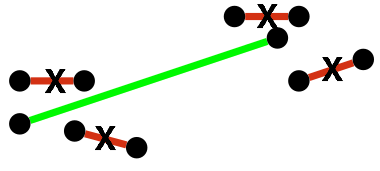
\includegraphics[scale=0.4]{gfx/ConstClust/Inform/Inform} 
	\caption[Ejemplo de conjunto de restricciones informativo.]{Ejemplo de conjunto de restricciones informativo. \cite{davidson2007survey}}\label{fig:figure16}
\end{figure}


La informatividad se estima utilizando el conjunto de restricciones como un conjunto de test, de manera que se mide la habilidad del algoritmo para predecir las restricciones presentes en él. Formalizando, dado un conjunto de restricciones $R$ y un algoritmo $A$, obtenemos la partición $P_A$ aplicando el algoritmo al conjunto de datos de entrada especificando el conjunto de restricciones vacío. Calculamos entonces la fracción de las restricciones incumplidas por $P_A$ \cite{davidson2007survey}:

\begin{equation}
I_A(R) = \frac{1}{|R|}\left[ \sum_{r \in R} unsat(r, P_A) \right] 
\end{equation}

\clearpage

Por otra parte, la \textbf{coherencia} mide el grado de concordancia dentro del propio conjunto de restricciones respecto a una métrica dada ($D$). Por ejemplo, la Figura \ref{fig:figure17} muestra dos restricciones paralelas y muy cercanas, pero de distinto tipo. Es en casos como este en los que se da una contradicción, ya que las restricciones \acf{ML} indican que la distancia entre las instancias involucradas en ellas es pequeña, mientras que las de tipo \acf{CL} deben indicar lo contrario.

\begin{figure}[!h]
	\centering
	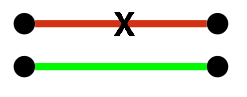
\includegraphics[scale=0.4]{gfx/ConstClust/Coherencia/Coher1}
	\caption[Ejemplo de conjunto de restricciones contradictorio.]{Ejemplo de conjunto de restricciones contradictorio. \cite{davidson2007survey}}\label{fig:figure17}
\end{figure}

Entonces, la medida de coherencia viene dada por el grado de solapamiento que presentan las restricciones al interpretarlas como vectores en el espacio y proyectarlas sobre uno de los ejes, tal y como se muestra en la Figura \ref{fig:figure18}.

\begin{figure}[!h]
	\centering
	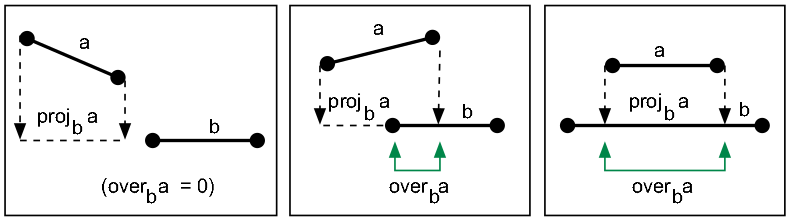
\includegraphics[scale=0.4]{gfx/ConstClust/Coherencia/Coher2}
	\caption[Representación de la medida de coherencia.]{Representación de la medida de coherencia. \cite{davidson2007survey}}\label{fig:figure18}
\end{figure}

\section{Resumen}

El clustering con restricciones incorpora nueva información al problema del clustering original, esta viene dada en forma de especificaciones de pertenencia al mismo o a diferentes clusters sobre parejas de instancias. Las restricciones, ya sean \acf{ML}, \acf{CL}, o restricciones de distancia, son utilizadas para guiar al método de clustering que apliquemos al conjunto de datos en cuestión, en la búsqueda de la partición resultado.

Los método de clustering derivados de este concepto han demostrado ser de gran utilidad en múltiples ámbitos, así como presenta problemas que pueden ser subsanados estudiando en profundidad las restricciones a emplear para resolver cada problema.


































